%!TEX options=--shell-escape
\documentclass[tikz]{standalone}
\usepackage[T1]{fontenc}
\usepackage[utf8]{inputenc}
\usepackage{xcolor}
\usepackage{amsmath}
\usepackage{amssymb}
\usepackage{hyperref}
\usepackage{accsupp}    
\usepackage{graphicx}
\usepackage{mathtools}
\usepackage{pagecolor}
\usepackage{amsmath} % for \dfrac
\usepackage{tikz,ifthen}
\tikzset{>=latex} % for LaTeX arrow head
\usepackage{braket}
\usepackage{pgfplots} 
\usepackage[edges]{forest}
\usetikzlibrary{patterns, backgrounds, arrows.meta}
\setlength{\parindent}{0cm}
\setlength{\parskip}{1em}

\usetikzlibrary{patterns, calc, intersections}

\def\rescale{0.1}
\def\innerwidth{25}
\def\outerwidth{53}
\def\innerlength{35}
\def\trackwidthmax{15}
\def\trackwidthmin{13}
\def\trackarcoffset{1}

\def\delta{2}


\begin{document}
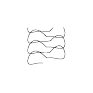
\begin{tikzpicture}[scale=\rescale]
\begin{axis}[
    view = {0}{60},
    axis lines = none,
    ymin = -8,
    ymax = 20,
    xmin = -8,
    xmax = 8
]

%\addplot3[thick, ->, domain=0:7*pi, samples=200, samples y = 0]({5 * sin(deg(-x)) + mod(x / pi, 2)}, {x}, {x});

\addplot3[thick, ->, domain=0:7*pi, samples=400, samples y = 0]({5 * sin(deg(-x)) + mod(x / pi, 2)}, {x + mod(2 * x / pi, 2) * 5 * sin(2 * deg(-x))}, {x});



\end{axis}

\end{tikzpicture} 
\end{document}

